\section{Preliminary Study}
\label{sec:preliminary}

In this section, we conduct an empirical analysis of tool-calling generation, covering (i) the latency breakdown between generation and tool execution, and (ii) analysis of tool-call patterns.

\begin{figure}[t]
\centering
\vspace{-0.5cm}
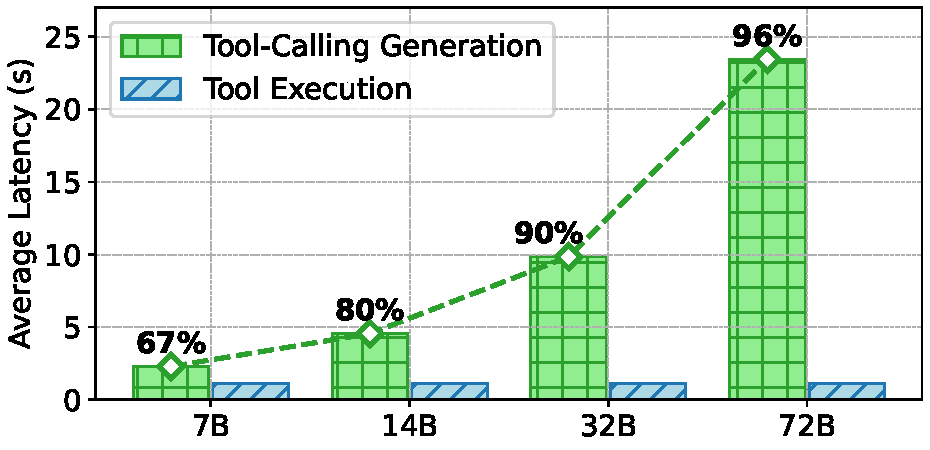
\includegraphics[width=0.95\columnwidth]{fig/latency_breakdown.pdf}
\caption{Latency breakdown of the Qwen2.5-Instruct model series on ToolBench~\citep{Qin:2024toolllm}. Tool execution latency remains essentially constant, whereas tool-calling generation latency increases with model scale, reaching up to $\bf 96\%$ of the end-to-end latency.}
\label{fig:latency_breakdown}
\end{figure}

\subsection{Latency Breakdown}
We begin by analyzing the latency bottlenecks in tool calling. Experiments are conducted using the Qwen2.5-Instruct series on ToolBench~\citep{Qin:2024toolllm}. As shown in Figure~\ref{fig:latency_breakdown}, tool execution latency remains nearly constant across model scales, whereas tool-calling generation latency increases significantly, accounting for up to $\bf{96\%}$ of the end-to-end latency for Qwen2.5-72B-Instruct. These results indicate that tool-calling generation is the dominant bottleneck in tool-calling pipelines, particularly in multi-tool, multi-turn scenarios, underscoring the importance of accelerating generation.

\subsection{Analysis of Tool-Call Patterns}
\label{sec:pattern_analysis}

Figure~\ref{fig:case} shows an example tool-calling trace from API-Bank~\citep{apibank}. As illustrated, these traces are highly structured JSON objects that conform to a constrained schema, consisting of:

\begin{itemize}
    \item \textbf{schema tokens}, e.g., \texttt{``name''}, \texttt{``parameters''}, and punctuation, which form the fixed scaffolding required by the tool-call schema;
    \item \textbf{tool and parameter names}, highlighted in \textcolor{myred}{red} and \textcolor{myblue}{blue}, respectively, which specify the target tool and its arguments;
    \item \textbf{parameter values}, in \textcolor{mygreen}{green}, which instantiate the arguments with query-specific content.
\end{itemize}

These structured patterns distinguish tool-calling generation from general natural-language generation, suggesting that it can be formulated as a \textit{constrained decoding} problem. In practice, valid tool calls must adhere to strict JSON schemas, implying that a large portion of the output tokens, i.e., schema tokens, is effectively predetermined. Once the target tool is selected, its parameter names are drawn from a finite, schema-defined set (e.g., \texttt{``user\_id''}, \texttt{``time''}, and \texttt{``health\_data''}). Consequently, the model only needs to generate a small subset of tokens, i.e., the parameter values, conditioned on the user query and the dialogue context.

\begin{figure}[t]
\centering
\vspace{-0.5cm}
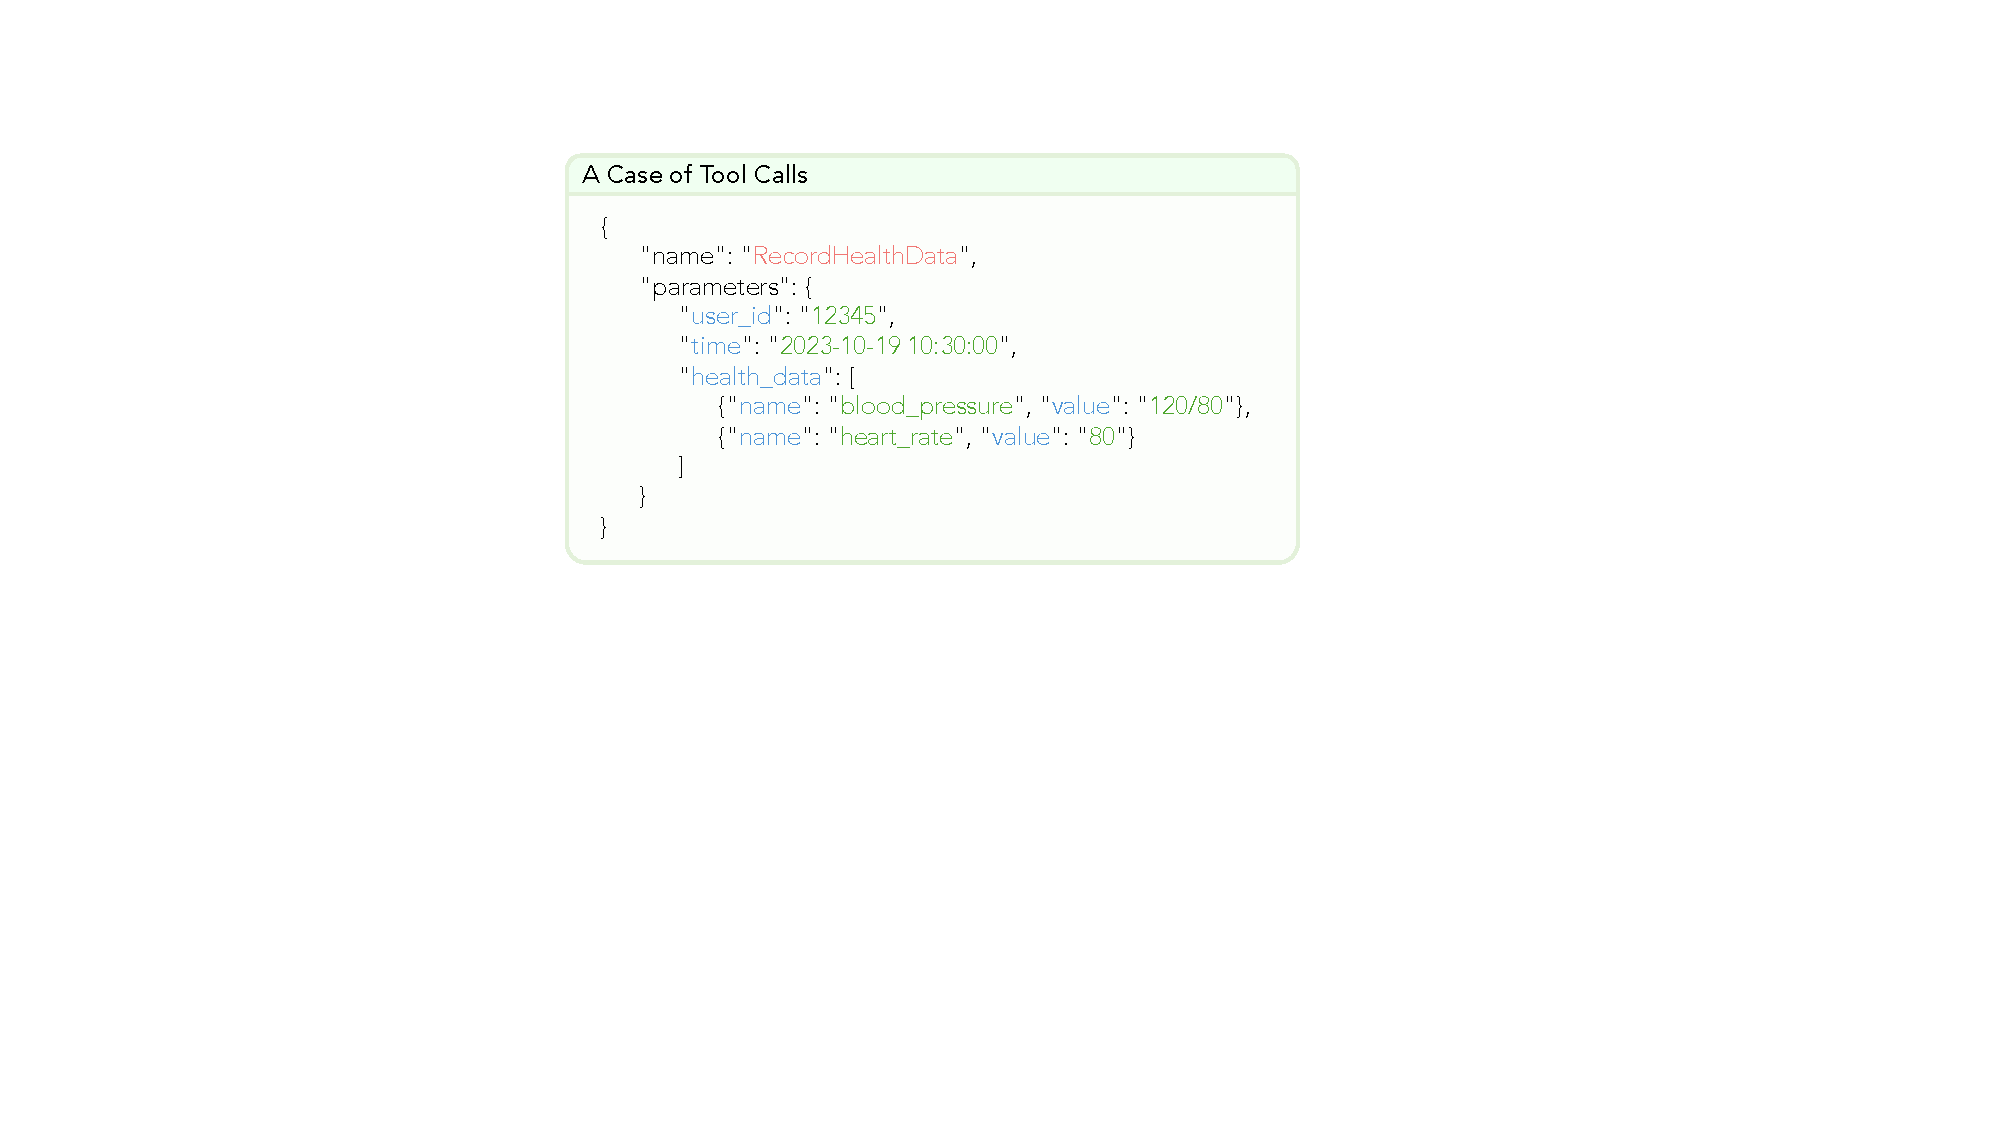
\includegraphics[width=0.95\columnwidth]{fig/case.pdf}
\caption{A tool-calling trace from API-Bank~\citep{apibank}, with different fields highlighted in color.}
\label{fig:case}
\end{figure}

In the following, we further analyze practical tool-calling behaviors in LLMs, including schema adherence and recurring tool-invocation patterns.

\begin{table}[t]
\centering
\small
%\resizebox{\linewidth}{!}{
\begin{tabular}{@{}lcc@{}}
\toprule
\bf Models & \bf API-Bank & \bf ToolAlpaca \\\midrule
Llama-3.1-8B-Instruct &$100.0\%$ &$100.0\%$\\
Llama-3.2-3B-Instruct &$99.5\%$ &$93.4\%$\\
Qwen2.5-14B-Instruct &$99.7\%$ &$100.0\%$\\
Qwen2.5-7B-Instruct &$100.0\%$ &$100.0\%$\\
\bottomrule
\end{tabular}%}
\caption{Format adherence of different models.}
\label{tab:format_adherence}
\end{table}

\paragraph{Schema Adherence}
As shown in Table~\ref{tab:format_adherence}, current tool-use LLMs exhibit strong adherence to tool-calling formats, i.e., their outputs can be reliably parsed as valid JSON. Both the LLaMA-Instruct and Qwen2.5-Instruct model families achieve over $99\%$ accuracy in following the required tool-call schema. This observation further supports our earlier claim that tool-calling generation can be formulated as constrained decoding under predefined schemas. In light of this, acceleration methods designed for general text generation may be suboptimal for tool calling. In contrast, explicitly exploiting the constrained structure of tool-calling generation can provide additional efficiency gains.

\begin{table}[t]
\centering
\vspace{-0.5cm}
\small
%\resizebox{\linewidth}{!}{
\begin{tabular}{@{}lccc@{}}
\toprule
\bf Datasets & \bf \#Tools & \bf \#Instances & \bf Avg. Tool Rep. \\\midrule
API-Bank &2138  &5221 & 10.95 \\
ToolAlpaca &426 &3938 & 4.82 \\
BFCLv2 & 739 &2251  & 9.01 \\
\bottomrule
\end{tabular}%}
\caption{Statistics of tool-calling benchmarks.}
\label{tab:tool_frequency}
\end{table}


\paragraph{Repetitive Tool Calls}
Beyond schema adherence, we observe that LLMs frequently invoke the same tools to satisfy recurring user intents and preference patterns. This behavior is consistently observed across widely used tool-calling benchmarks. As shown in Table~\ref{tab:tool_frequency}, repeated invocations of identical tools occur frequently in API-Bank~\citep{apibank}, with the average number of calls per tool exceeding $10.95$. This observation motivates exploiting historical tool-calling traces. Rather than discarding prior calls, a system can reuse previously issued tool calls when they remain valid, thereby further improving tool-calling efficiency.